\documentclass{beamer}
\usepackage{ucs}
\usepackage{url}
\usepackage{graphicx}
\usepackage[utf8x]{inputenc} % ou utf8x au lieu
\usepackage[T1]{fontenc} % de latin 1
\usepackage{lmodern}
\usepackage[french]{babel}
\usepackage{listings}
\renewcommand{\familydefault}{\sfdefault}

\usetheme{Singapore}
\beamertemplatenavigationsymbolsempty
\setbeamerfont{page number in head/foot}{size=\footnotesize}
\setbeamertemplate{footline}[frame number]

\title{{\huge Eurobot 2015, BetterWithMotors}} 
\author{José-Carlos Alves Da Costa\\
	Mounïme Bouzanih\\
	Louis Defauw\\
	Arnaud Iserentant\\
	Abdelhak Kotati\\
	Nabil Nehri\\
	Alexis Paques}
\date{\today}
\begin{document}

\maketitle

\begin{frame}
\frametitle{Introduction}
\begin{itemize}
	\item Gestion du projet;
	\item Table et actions du robot;
	\item Architecture;
	\item Communication entre les cartes;
	\item Régulation des moteurs;
	\item Châssis;
	\item Pince;
	\item Moteurs et drivers;
	\item Perspectives.
\end{itemize}
\end{frame}

\begin{frame}
\frametitle{Gestion}
\begin{description}
	\item[Méthode SCRUM] 
	\item Stand-Up meeting avec tournante d'animateur;
	\item Délivrables à court et à long terme;
	\item Travail en binôme la plupart du temps;
	\item Avantages/Inconvénients.
	\item[Git]
	\item Important d'être à jour;
	\item Avantages/Inconvénients.
\end{description}
\end{frame}
%Table & actions
\subsection{Table}
%~~~~~~~~~~~~~~~~~~~~~~~~~~~~~~~~~~~~~~~~~~~~~~~~~~~~~~~~~~~~
\paragraph{}
La réalisation de la table fut l'un des premiers objectifs cruciaux à atteindre. 

\noindent En effet, requérant un investissement important de temps, la table est essentielle pour avoir une idée visuelle des actions que devront réaliser les robots et donc permettre de tester les prototypes en situation réelle. On peut ajouter également qu'avoir un élément physique terminé donne l'agréable sensation d'être sur le bon chemin et redonne du cœur à l'ouvrage.

\paragraph{}
Sa mise en œuvre fut divisée en plusieurs étapes : 
\begin{itemize}
	\item Achat des matériaux : peinture, bois et vis;
	\item Découpe des planches;
	\item Assemblage;
	\item Peinture;
	\item Tracés des détails : ligne noire, logo, etc..
\end{itemize}

\paragraph{}
La production se déroula sur les premiers mois du projet (octobre à novembre).

\noindent Après la livraison des planches découpées à la fin de la semaine de Toussaint (03/11), l'équipe s'est relayée pour effectuer l'assemblage et la peinture des différents éléments.

\noindent La réalisation de la table ne posa aucun problème majeur hormis un détail : La dimension d'épaisseur requise des planches (20mm) n'est pas une norme belge et ne pouvait être négligée, car elle sert, entre autre, à réaliser les marches de l'escalier. Cela impliqua un délai supplémentaire lors de la commande retardant inévitablement la découpe. Le résultat est visible sur la figure~\ref{img:table}.

\begin{figure}[!ht]
	\centering
	\includegraphics[width=15cm]{Eurobot_Table_1.JPG}
	\caption{Table}
	\label{img:table}
\end{figure}

\subsection{Action des robots}
%~~~~~~~~~~~~~~~~~~~~~~~~~~~~~~~~~~~~~~~~~~~~~~~~~~~~~~~~~~~~
\subsubsection{Introduction}
%~~~~~~~~~~~~~~~~~~~~~~~~~~~~~~~~~~~~~~~~~~~~~~~~~~~~~~~~~~~~
Chaque match est composé de 5 épreuves à réaliser grâce à 1 ou 2 robots indépendants. Aucun contact entre les adversaires n’est autorisé sous peine de malus donc les robots devront être prompts à s’arrêter en cas de rencontre.

\subsubsection{The spotlight}
%~~~~~~~~~~~~~~~~~~~~~~~~~~~~~~~~~~~~~~~~~~~~~~~~~~~~~~~~~~~~
Le robot devra bâtir des spotlights. Pour ce faire, il devra aller récupérer des stands de sa couleur (8 au total) et les amener dans une des zones de construction (1 par équipe + 1 commune).  Ensuite, il suffira d’empiler les stands le plus haut possible et de placer une balle de tennis (4 disponibles, mais communes aux 2 équipes) à son sommet.

\noindent Chaque stand présent dans la zone de construction personnelle rapportera des points mais un seul spotlight peut y être construit. Les autres devront être réalisés dans la zone commune.

\noindent On ne peut en aucun cas interagir avec les stands adverses et un spotlight placé sur la plateforme de la zone commune ne peut être altéré (vol de la balle de tennis) par l’adversaire.

\paragraph{}
Chaque plot rapporte 2 points s’il est correctement placé dans une zone de construction et 3 points bonus par spotlight valide (tour avec balle de tennis).

\subsubsection{The clapperboards}
%~~~~~~~~~~~~~~~~~~~~~~~~~~~~~~~~~~~~~~~~~~~~~~~~~~~~~~~~~~~~
Le robot devra aller fermer les clapperboards correspondant aux couleurs de son équipe qui sont au nombre de 3 (2 proches de sa zone de départ et 1 chez l’adversaire). Il peut se servir de la ligne noire tracée au sol pour se diriger facilement jusqu’aux clapperboards.

\paragraph{}
Cette épreuve rapporte 5 points par clapperboard correctement fermé.

\subsubsection{The popcorn}
%~~~~~~~~~~~~~~~~~~~~~~~~~~~~~~~~~~~~~~~~~~~~~~~~~~~~~~~~~~~~
Le robot devra récolter des popcorns et soit les amener dans sa base et les placer dans la rigole de récupération soit les placer dans un gobelet et l’amener dans une des 3 zones « cinéma » appartenant à son équipe (1 gobelet maximum par zone, le plus rempli sera pris en compte). 

\noindent Les popcorns sont initialement mis dans les gobelets ou dans les machines de distribution. La table proposera 5 verres contenant chacun 4 popcorns et 4 machines avec 5 popcorns.

\noindent Il est nécessaire de savoir que les gobelets placés dans un cinéma peuvent être « volés » par l’équipe adverse.

\paragraph{}
Chaque popcorn présent dans un gobelet placé dans une zone « cinéma » ou placé dans la rigole de la base rapportera 1 point.

\subsubsection{Climbing the red carpet steps}
%~~~~~~~~~~~~~~~~~~~~~~~~~~~~~~~~~~~~~~~~~~~~~~~~~~~~~~~~~~~~
Le robot devra se diriger vers les escaliers situés à l'arrière de la zone de jeu, gravir les marches pour se trouver au sommet à la fin du match.

\paragraph{}
15 points seront attribué en cas de réussite.

\subsubsection{The red carpet}
%~~~~~~~~~~~~~~~~~~~~~~~~~~~~~~~~~~~~~~~~~~~~~~~~~~~~~~~~~~~~
Le robot devra placer de part et d’autre de son escalier un bout de tissu rouge sur les marches de couleurs grises. Pour ce faire, le plus simple sera de monter au sommet et, ensuite, de dérouler le tissu préalablement roulé et mis à bord du robot. 

\paragraph{}
Chaque marche (4 au total x 2) couverte rapportera 2 points et un bonus de 4 points sera offert par volée complètement couverte.

\subsubsection{Bonus/Malus}
%~~~~~~~~~~~~~~~~~~~~~~~~~~~~~~~~~~~~~~~~~~~~~~~~~~~~~~~~~~~~
Toute pénalité impliquera un retrait de 10 points à l'équipe jusqu'à un minimum de 0.
\noindent Il est important se savoir que pour valider un point, le robot ne peut plus avoir d'emprise sur l'objet en question : si en déplacant le robot sur son axe de déplacement principal en impliquant un mouvement de l'objet, celui-ci ne sera pas valide.
\noindent Et, pour finir, 5 points seront attribués à chaque équipe qui n'est pas considérée comme "scratched" : robot présent et fonctionnel.

\subsubsection{Situation Actuelle}
%~~~~~~~~~~~~~~~~~~~~~~~~~~~~~~~~~~~~~~~~~~~~~~~~~~~~~~~~~~~~
Dans notre cas, nous alignerons 2 robots qui s'occuperont chacun de plusieurs tâches distinctes. 

\noindent Le principal s'occupera des 3 premières épreuves : The spotlight, The clapperboards et The popcorn. Tandis que le second s’occupera des escaliers : Climbing the red carpet steps et The red carpet.

\paragraph{}
Pour assurer ces deux dernières opérations, le choix s’est orienté vers l’achat d’un robot à chenille déjà assemblé compatible avec arduino. Nous l’avons choisi notamment pour sa bonne répartition du poids et sa facilité à franchir les marches d’escalier.  

\paragraph{}
Pour le moment, notre attention est dirigée sur The clapperboards et Climbing the red carpet steps qui, en plus de rapporter une bonne quantité de points sans trop de difficulté (3*5 + 15 points), parcoure l'ensemble des fonctionnalités primaires attendues chez nos 2 robots à savoir le déplacement, la détection et la gestion des obstacles, la maitrise de la pince mécanique et l'escalade des marches.

\noindent Pour les autres épreuves, nous n’avons pas encore déterminé l’ordre des actions que le robot effectuera et comment il devra réagir en situation réelle.
%Architecture
\subsection{Buts principaux}
%~~~~~~~~~~~~~~~~~~~~~~~~~~~~~~~~~~~~~~~~~~~~~~~~~~~~~~~~~~~~
L'architecture hardware du robot a pour objectif d'être modulable. Cette solution a été retenue afin de pouvoir ajouter des fonctionnalités supplémentaires au cours du projet. L'avantage principal est d'avoir la possibilité de se concentrer sur un module à la fois.

\noindent Quatre modules ont été définis pour permettre au robot de réaliser les actions de bases. Chacun, basé sur une carte électronique propre, sera connecté à la carte principale via un bus de communication (I2C, SPI ou UART). Les modules sont les suivants :

\begin{itemize}
	\item Arduino Master : carte principale qui contrôlera l'ensemble du robot. Elle est à la tête de toutes les autres cartes.;
	\item Arduino Motor : module très important qui commandera les moteurs ;
	\item Raspberry Pi : module qui aura  pour but de voir ce qu'il se passe autour du robot afin de définir les objectifs à atteindre.;
	\item Arduino Bras : carte secondaire qui contrôlera la pince du robot.
\end{itemize}

\paragraph{}
Le fait que l'architecture soit modulable permettra également aux futurs utilisateurs de récupérer un ou plusieurs module pour les exploiter dans leur projet.

\noindent On peut voir les liens entre les différents modules sur la figure~\ref{img:hardware}. On y voit également des éléments tels que la batterie, les moteurs, ou encore les différents capteurs présents sur le robot. Il faut cependant bien avoir en tête que ce schéma n'est qu'une version provisoire qui évoluera avec le projet.

\begin{figure}[!ht]
	\centering
	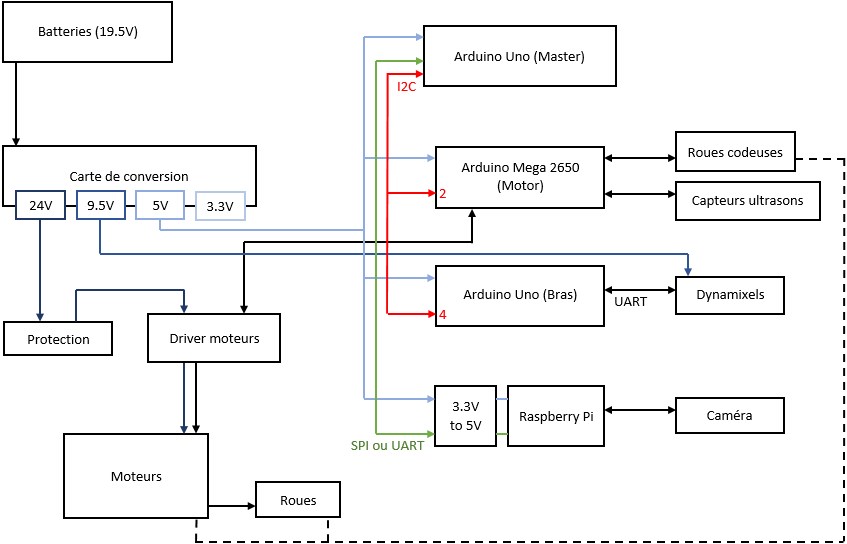
\includegraphics[width=15cm]{hardware.PNG}
	\caption{Schéma bloc hardware}
	\label{img:hardware}
\end{figure}

\subsection{Choix des cartes}
%~~~~~~~~~~~~~~~~~~~~~~~~~~~~~~~~~~~~~~~~~~~~~~~~~~~~~~~~~~~~
Pour notre robot, nous avons ensemble énuméré les avantages et désavantages de chacune des cartes pour nous faciliter la tâche quand nous devrons les utiliser.

\noindent On peut travailler avec une Rasperry Pi, une Arduino ou encore une DE0 nano, mais quelle est la meilleure ? 

\subsubsection{DE0 nano}
%~~~~~~~~~~~~~~~~~~~~~~~~~~~~~~~~~~~~~~~~~~~~~~~~~~~~~~~~~~~~
\noindent Avantages :
\begin{itemize}
	\item Instantanée;
	\item Carte plus performante que les autres (très puissante);
	\item Nombreuses pins à disposition.
\end{itemize}

\noindent Inconvénients :
\begin{itemize}
	\item Difficulté lors de la programmation (VHDL);
	\item Coût important;
	\item Test Bench à faire manuellement;
	\item Limitée par le nombre de sorties;
	\item Temps de compilation plus lent que les autres cartes.
\end{itemize}

\subsubsection{Raspberry Pi}
%~~~~~~~~~~~~~~~~~~~~~~~~~~~~~~~~~~~~~~~~~~~~~~~~~~~~~~~~~~~~
\noindent Avantages :
\begin{itemize}
	\item Utilisation facile, architecture linux;
	\item Utilisation de la caméra aisée;
	\item OpenCV, très bien documenté.
	\item Elle freeze (Testé en laboratoire).
\end{itemize}

\noindent Inconvénients :
\begin{itemize}
	\item Limitation du nombre pins, besoin d'une carte supplémentaire;
	\item Système exploitation, implique que l'on est pas en temps réel; 
	
\end{itemize}

\subsubsection{Arduino}
%~~~~~~~~~~~~~~~~~~~~~~~~~~~~~~~~~~~~~~~~~~~~~~~~~~~~~~~~~~~~
\noindent Avantages :
\begin{itemize}
	\item Consommation faible : 42mA (0,5W) pour 700mA (3,5W) sur Rpi;
	\item Temps réel (ATmega328 8 bits d'Atmel à 16MHz);
	\item Communautaire et très documentée sur internet;
	\item Programmation aisée en C++;
	\item Communication : module pré-existant.
\end{itemize}

\noindent Inconvénients :
\begin{itemize}
\item 32 Ko d'espace mémoire uniquement (Uno);
\item Impossibilité d'intégrer un module caméra avec une Arduino.
\end{itemize}

\subsection{Nomenclature}
%~~~~~~~~~~~~~~~~~~~~~~~~~~~~~~~~~~~~~~~~~~~~~~~~~~~~~~~~~~~~
Cette liste nous permet d'avoir une vue d'ensemble de ce que nous allons utiliser comme matériel. Cependant, elle n'est pas définitive. En effet, elle sera sujette à quelques modifications (ajout et/ou suppression d'éléments) tout au long du projet. 

\noindent Liste : 
\begin{enumerate}
	\item Roues : 
	\begin{itemize}
		\item 2 roues;
		\item 2 roues codeuses;
		\item Buffer 3,3-5V;
		\item Roue libre.
	\end{itemize}

	\item Moteur : 
	\begin{itemize}
		\item 2 moteurs;
		\item 4 engrenages;
		\item 2 courroies;
		\item Drivers.
	\end{itemize}

	\item  Cartes : 
	\begin{itemize}
		\item Raspberry Pi;
		\item 2 Arduino Uno;
		\item DE0 nano;
		\item Arduino Mega 2560;
		\item Carte ECAM RPI (Buffer);
		\item Carte stratégie, initialisation et démarrage avec corde;
		\item Bouton arrêt urgence.
	\end{itemize}

	\item Alimentation : 
	\begin{itemize}
		\item Carte ECAM.
	\end{itemize}

	\item Capteurs : 
	\begin{itemize}
		\item Line tracking;
		\item 2 Gyroscopes accéléromètre;
		\item 5 Capteurs ultrasonique.
	
	\end{itemize}

	\item Châssis : 
	\begin{itemize}
		\item Vis (quincaillerie);
		\item 3 plaques acier;
		\item Tiges;
		\item Courroie-Poulie;
		\item Plexiglas (carrosserie). 
	\end{itemize}

	\item Système levage pince : 
	\begin{itemize}
		\item Pince modèle ECAM ;
		\item Rail ;
		\item 3 Dynamixel;
		\item 2 poulies crantée avec roulement à billes;
		\item Courroie crantée;
		\item 1 plaque en L pour fixer la Dynamixel du la courroie sur structure.
	\end{itemize}
\end{enumerate}
\begin{frame}
\frametitle{Communications}
\framesubtitle{Arduino - Arduino}

\begin{description}
\item[I\up{2}C]
\item Transfert à plusieurs esclaves;
\item Fonction;
\item Données.
\end{description}

\begin{table}[!ht]
	\centering
	\begin{tabular}{|c|c|c|c|}
		\hline
		adresse & fonction & data & data \\
		\hline
		7 bits & 4 bits & 4 bits & 8 bits \\
		\hline
	\end{tabular}
	\caption{Trame I\up{2}C}
	\label{tb:TrameI2C}
\end{table}
\end{frame}

\begin{frame}
\frametitle{Communications}
\framesubtitle{Arduino - DE0nano}
\begin{description}
\item[Direct]
\item Appliquer un prescaler;
\item Transfert d'un signal.
\end{description}
\end{frame}

\begin{frame}
\frametitle{Communications}
\framesubtitle{Arduino - Raspberry Pi}
\begin{description}
\item[SPI/UART]
\item Communication entre 2 cartes;
\item Transfert de données.
\end{description}
\end{frame}

\begin{frame}
\frametitle{Régulation}
\framesubtitle{Introduction}
Quelques questions à se poser :
\begin{itemize}
	\item Où veut-on aller ?
	\item Comment commander les moteurs ?
	\item Vers où le robot se dirige-t-il ? Où est-il par rapport à l'objectif ?
	\item Il y a-t-il un obstacle devant le robot ?
	\item Pourquoi a-t-on besoin d'une régulation ?
\end{itemize}
\end{frame}

\begin{frame}
\frametitle{Régulation}
\framesubtitle{Consigne et commande des moteurs}
La consigne est reçue via l'I\up{2}C, on a disposition :
\begin{itemize}
	\item La fonction (4bits), choix de la commande;
	\item Les données (12bits), distance à parcourir.
\end{itemize}
\begin{table}[!ht]
	\centering
	\begin{tabular}{|l|cc|cc|}
		\hline
		& DIR1 & DIR2 & PWM1 & PWM2 \\
		\hline
		Forward & 1 & 1 & \multicolumn {2}{c|}{Variable} \\
		\hline
		Backward & 0 & 0 & \multicolumn {2}{c|}{Variable} \\
		\hline
		Turn Left & 1 & 0 & \multicolumn {2}{c|}{Variable} \\
		\hline
		Turn Right & 0 & 1 & \multicolumn {2}{c|}{Variable} \\
		\hline
		Stop & \multicolumn {2}{c|}{X} & 0 & 0 \\
		\hline
	\end{tabular}
	\caption{Commandes des moteurs}
\end{table}
\end{frame}

\begin{frame}
\frametitle{Régulation}
\framesubtitle{Roues codeuses et capteurs ultrasons}
Capteurs ultrasons : uniquement en cas d'arrêt d'urgence.\\
Roues codeuses :
\begin{itemize}
	\item 1024 tics par tour ;
	\item 20 cm par tour.
\end{itemize}
\begin{figure}[!ht]
	\centering
	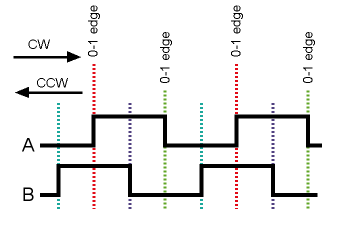
\includegraphics[scale=0.5]{roues_codeuses.png}
	\caption{Signal des roues codeuses}
\end{figure}
\end{frame}

\begin{frame}
\frametitle{Régulation}
\framesubtitle{Schéma bloc}
\begin{figure}[!ht]
	\centering
	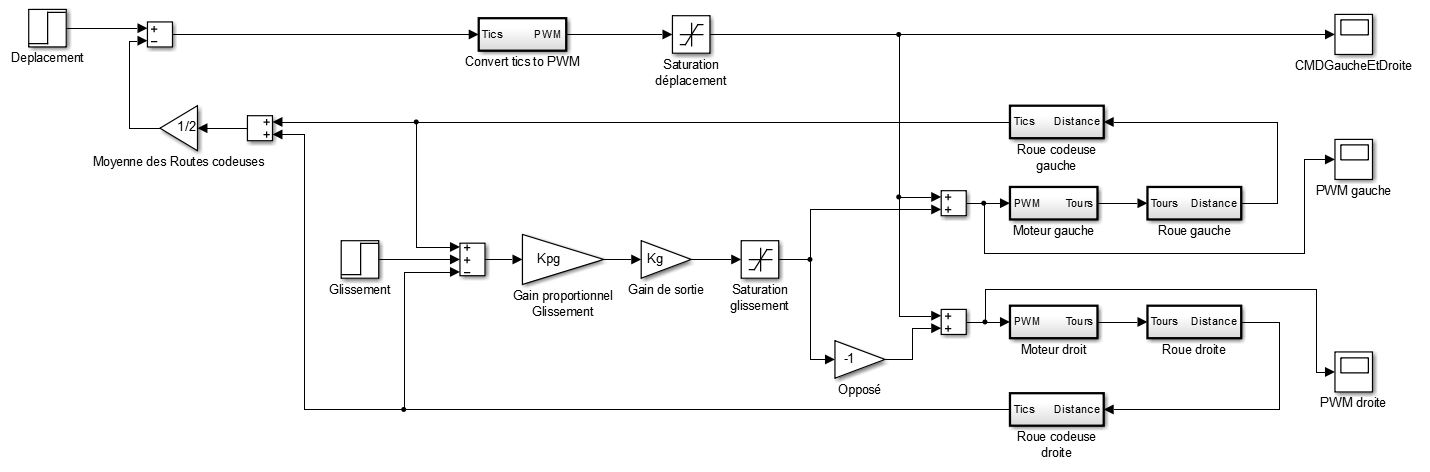
\includegraphics[scale=0.28]{simulink.jpg}
	\caption{Schéma bloc de la régulation des moteurs}
	\label{img:simulink}
\end{figure}
\end{frame}

\begin{frame}
\frametitle{Régulation}
\framesubtitle{Coefficients Kp et Kig}
\begin{description}
	\item[Kp] Coefficient proportionnel du déplacement; 
			\hfill \\ Ralentir la commande en se rapprochant. 
	\item[Kig] Coefficient intégrateur du glissement;
			\hfill \\ Éviter les variations entre la rotation des moteurs et la rotation des roues.
\end{description}
\end{frame}
\begin{frame}
\frametitle{Châssis et conceptions mécaniques}
\framesubtitle{Objectifs}
Conception d'une base adéquate capable de recevoir une pince mécanique et les nouveaux moteurs acquis cette année. 
\end{frame}

\begin{frame}
\frametitle{Châssis et conceptions mécaniques}
\begin{figure}[!ht]
	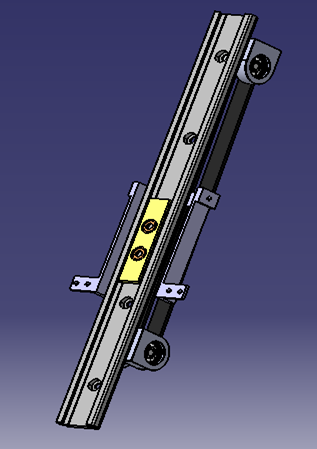
\includegraphics[scale=0.5]{chariot.png} 
	\caption{Mécanisme d'élévation}
\end{figure}
\end{frame}

\begin{frame}
\frametitle{Châssis et conceptions mécaniques}
\begin{figure}[!ht]
	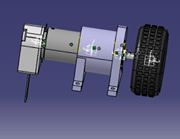
\includegraphics[scale=0.5]{support.jpg}
	\caption{Support moteur} 
\end{figure}
\end{frame}

\begin{frame}
\frametitle{Châssis et conceptions mécaniques}
\begin{figure}[!ht]
	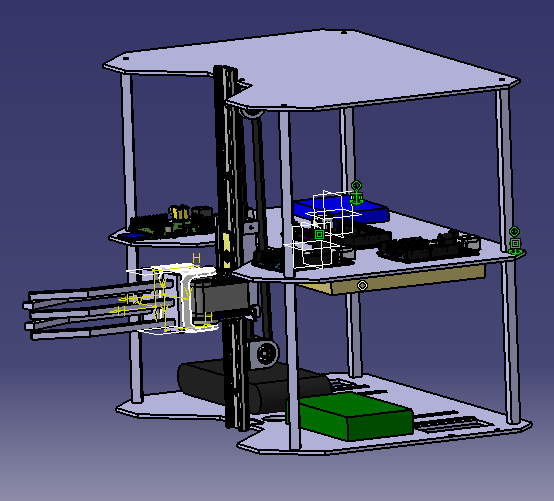
\includegraphics[scale=0.5]{assemblage.png}
	\caption{Assemblage des différents éléments} 
\end{figure}
\end{frame}

\begin{frame}
\frametitle{Châssis et conceptions mécaniques}
\framesubtitle{Inconvénients}
\begin{itemize}
	\item Une seule action à la fois;
	\item Le positionnement correct du robot face à l'objet;
	\item L'encombrement de la pince.
\end{itemize}
\end{frame}

%Pince et dynamixel
\subsection{Servomoteurs - Dynamixel AX12}
\subsubsection{Caractéristiques}
\begin{itemize}
    \item Un servomoteur est un système asservi capable de maintenir une opposition à un effort statique; 
    \item C’est donc une sorte de moteur qui est capable d’atteindre une vitesse et un angle déterminé;
    \item On transmet au servomoteur des ordres sous forme d'une modulation à largeur d’impulsion appelée PWM;
    \item On envoi une impulsion et c’est le temps de l’impulsion qui détermine l’angle à fournir par les servomoteurs;
    \item Pour comprendre son utilisation je vais rappeler certaines de ces caractéristiques.
\end{itemize}

\begin{figure}[!ht]
    \centering
    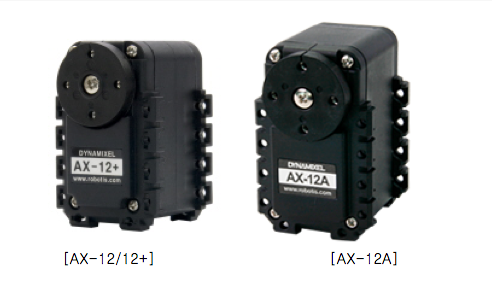
\includegraphics[scale=0.5]{AX.png}
    \caption{Dynamixels}
    \label{img:AX12}
\end{figure}

\paragraph{Caractéristiques du modèle AX12}
\begin{itemize}
    \item Poids : 54,6g;
    \item Dimension : 32mm * 50mm * 40mm;
    \item Angle autorisé : 0 à 300°;
    \item Résolution : 0.29°;
    \item Tension alimentation : 9 ~ 12V ;
    \item Type Protocole : Half duplex Asynchronous Serial Communication (8bit,1stop,No Parity);
    \item ID : de 254 identifiants possibles;
    \item Lecture possible : T°, tension, position.
\end{itemize}

\paragraph{Angle limite}

\begin{figure}[!ht]
    \centering
    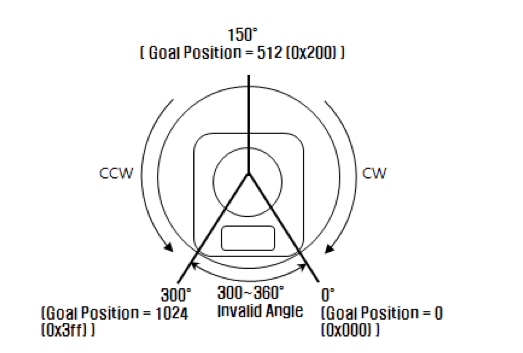
\includegraphics[scale=0.4]{angle.png} 
    \caption{Angle limite de la dynamixel}
    \label{img:angle_AX12}
\end{figure}

On peut aisément visualiser la position du 0° et la course possible du servomoteur sur la figure~\ref{img:angle_AX12}. Quand nous donnons une valeur d’angle nous la donnons de 0 à 1023 ce qui correspond à une valeur d’angle entre 0 et 300 °. Si je veux 150° je dois envoyer la valeur de 511,5 et mon servomoteur se positionnera en réalité à la position de notre 0 conventionnel. Si nous l’utilisons en « Wheel Mode » le servomoteur peut tourner sur 360° sans problème. 

\paragraph{Vitesse}
\subparagraph{Join Mode}
Nous envoyons une valeur entre 0 et 1023 où 1023 est la vitesse maximale du servomoteur. L’unité vaut 0,111rpm et la vitesse maximale est de 0,111*1023 = 113,553rpm (rotations par minute).
\subparagraph{Wheel mode}
En Wheel mode il faut connaitre la notion de CCW et CW qui correspondent respectivement à la rotation en sens anti horaire et la rotation en sens horaire. On peut utiliser des valeurs entre 0 et 2047. 

\subsection{Utilisation}
Pour utiliser les servomoteurs il faut d’abord intégrer la librairie "DynamixelSerial.h". Cette librairie contient toutes les fonctions déjà faites qui nous seront utiles pour utiliser
les servomoteurs. 

\noindent Notre objectif est de parcourir la liste et de se familiariser avec les différentes possibilités. 

\noindent Je vais tout d’abord décrire un certain nombre d’entre elles. 

\begin{enumerate}
     \item Dynamixel.begin(BaudRate, RxPin, TxPin, DataControl) \begin{itemize}
         \item On initialise la communication série avec l’arduino;
         \item RxPin est la pin de réception de données et TxPin pour la transmission de données.
     \end{itemize}
     
     \item Dynamixel.ping(ID)
     \begin{itemize}
        \item Connaître le statut du servomoteur.
     \end{itemize}
      
     \item Dynamixel.reset(ID)
     \begin{itemize}
        \item Rétablir les réglages par défaut du Dynamixel.
     \end{itemize}
      
     \item Dynamixel.setID(ID, new ID )
     \begin{itemize}
        \item Change l’ID du servomoteur.
     \end{itemize}
     
     \item Dynamixel.move(ID ,Position)
     \begin{itemize}
        \item Déplace la dynamixel jusqu’à la position correspondante, de 0 à 1023.
     \end{itemize}
     
     \item Dynamixel.movespeed(ID,Position,Speed)
     \begin{itemize}
        \item On précise en plus la vitesse voulue.
     \end{itemize}
     
     \item Dynamixel.moveRW(ID,Position)
     \begin{itemize}
        \item Enregistre l’instruction qui déplace le mécanisme jusqu’à une position correspondante.
     \end{itemize}
     
     \item Dynamixel.moveSpeedRW(ID,Position,Speed)
     \begin{itemize}
        \item Enregistre l’instruction.
     \end{itemize}
     
     \item Dynamixel.action()
     \begin{itemize}
        \item Exécute l’instruction sauvegardée dans le servo.
     \end{itemize}
     
     \item Dynamixel.setEndless(ID,Status)
     \begin{itemize}
        \item Active ou désactive la rotation en continue du servomoteur;
        \item Statut : ON/OFF.
     \end{itemize}
     
     \item Dynamixel.turn(ID,Side,Speed)
     \begin{itemize}
         \item ID - Identifiant Servomoteur;
         \item Sens de rotation RIGHT/LEFT;
         \item Speed : Vitesse de 0 à 1023.
     \end{itemize}
     
     \item Dynamixel.torqueStatus(ID,Status)
     \begin{itemize}
        \item Active ou désactive le mode couple du servomoteur.
     \end{itemize}
     
     \item Dynamixel.LEDStatus(ID,Status)
     \begin{itemize}
        \item Active ou désactive la LED.
     \end{itemize}
     
     \item Dynamixel.readPosition(ID)
     \begin{itemize}
        \item Renvoi  la valeur de la position.
     \end{itemize}
     
     \item Dynamixel.readSpeed(ID)
     \begin{itemize}
        \item Renvoi la vitesse en RPM.
     \end{itemize}
\end{enumerate}

\subsection{Pince}
Cette année notre robot devra effectuer certaines tâches nécessitant l’utilisation d’une pince. Nous avons tout d’abord cherché à savoir ce qui existait déjà dans le commerce. Mais nous avons très vite renoncé à cette idée en se basant sur 2 réflexions : 

\begin{itemize}
    \item Prix d’achat trop élevé;
    \item Utilisation des Dynamixel déjà étudiée lors du projet Eurobot or la plupart des pinces fonctionnent avec des servomoteurs d’un autre type. Il aurait fallu tout recommencer.
\end{itemize}

\paragraph{}
En partant sur cette réflexion nous nous sommes rapidement lancés dans la conception de notre propre pince qui serait imprimée grâce à l’imprimante 3D. Les objets à porter sont :

\begin{itemize}
\item Verres simples;
\item Plots en bois ;
\item Balles en polystyrène.
\end{itemize}

\paragraph{}
Il nous faudra donc une pince classique avec deux doigts qui se referment. Nous étions partis là-dessus lors de la conception mais j’ai pensé à réutiliser le système des pinces à cheveux qui se referment. En croisant les doigts comme la pince à cheveux on pourra mieux attraper les objets comme des balles de ping pong.

\begin{figure}[!ht]
    \centering
    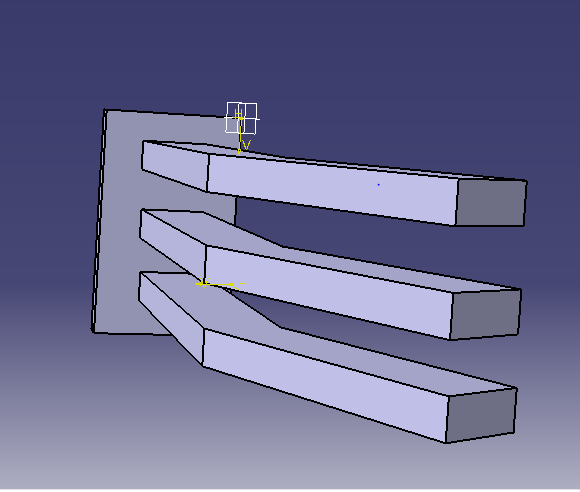
\includegraphics[scale=0.5]{pince2.png}
    \caption{Pince faite sur Catia, partie de gauche}
\end{figure}

\begin{figure}[!ht]
    \centering
    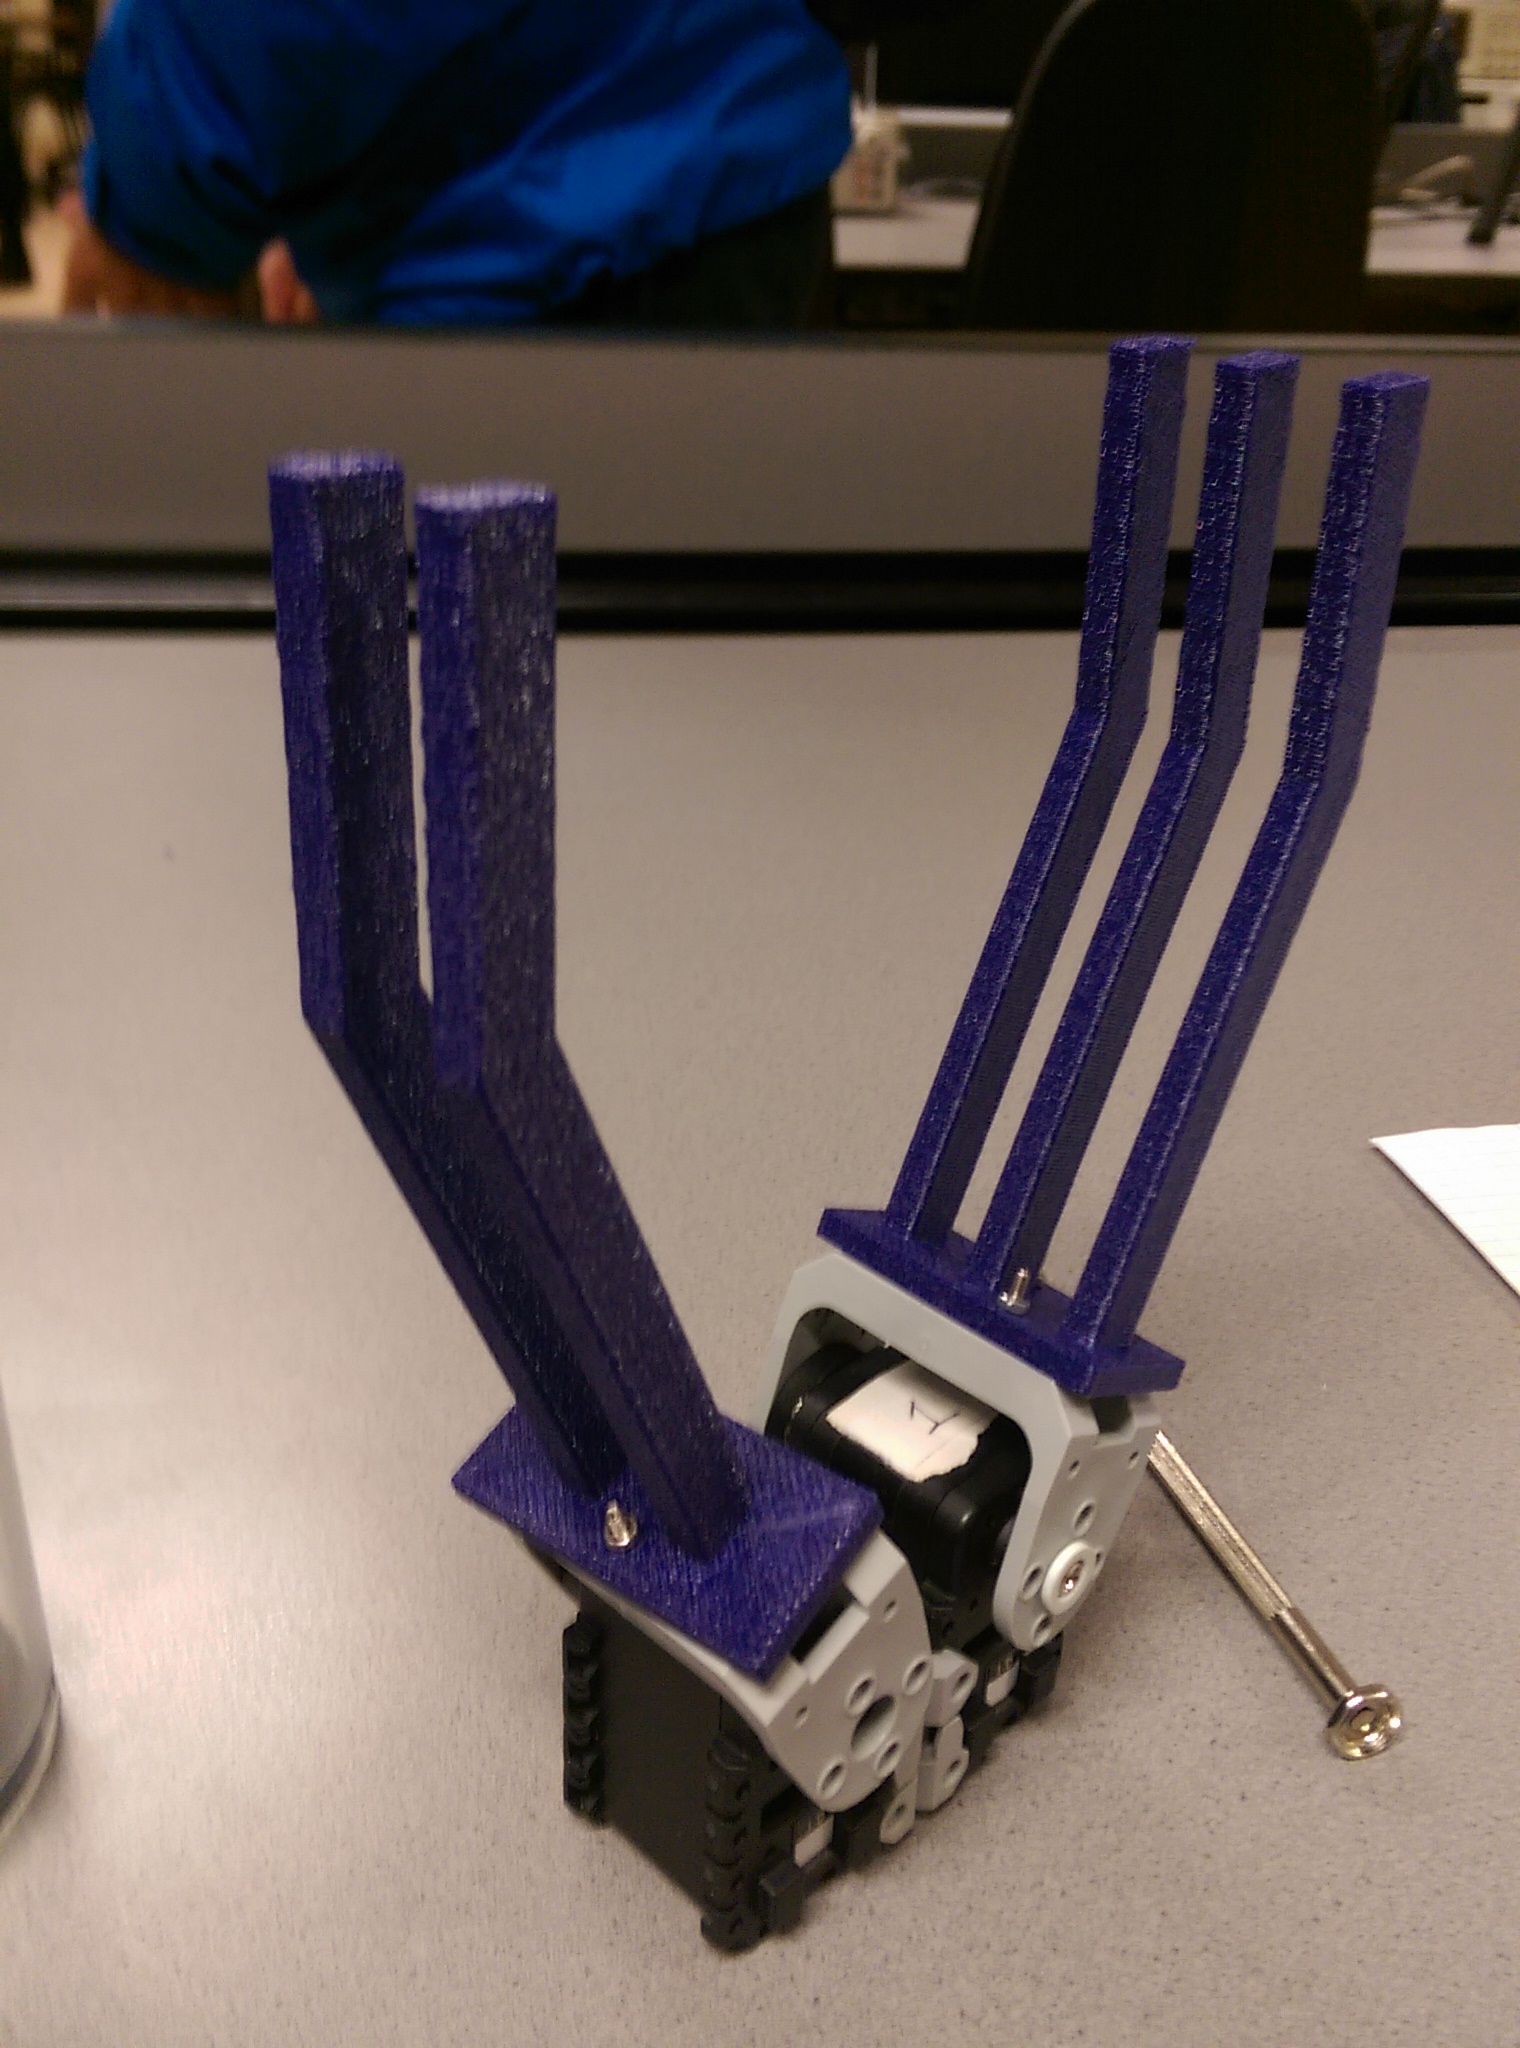
\includegraphics[width=10 cm]{pince1.jpg}
    \caption{Prototype de la pince (version légère}
    \label{fig:Pince1}
\end{figure}

\noindent Cette version qui est devenue la version finale a donc 3 doigts à droite et 2 doigts à gauches capables de se croiser (figure~\ref{fig:Pince1}). Les deux côtés sont chacun reliés à une Dynamixel qui sera contrôlée par une Arduino.

\noindent Cette pince sera elle même accrochée sur un rail qui lui permettra de faire des déplacements verticaux. La courroie sera guidée par une 3\up{ème} Dynamixel. On pourra ainsi faire monter, descendre, ouvrir et fermer selon un angle bien précis la pince grâce aux fonctions étudiées plus haut. 
Toute l'étude des couples et des objets à porter sera étudiée plus tard.
\begin{frame}
\frametitle{Moteur}
\framesubtitle{Dimensionnement}
\begin{description}
\item[Régime permanent]
\item En régime permanent l'accélération est nulle;
\item $Fm - Fr = m \times \overrightarrow{a} = 0$.
\item[Résultats]
\item $P = Cm \times \omega m = 694\frac {rad}{s}  \times 0.02943N = 20.42W$;
\item Vitesse maximale du robot $V = 5\frac{km}{h} = 1.38\frac{m}{s}$.
\end{description}
\end{frame}

\begin{frame}
\frametitle{Moteur}
\framesubtitle{Dimensionnement en tenant compte de l'accélération}
\begin{itemize}
\item Pour simplifier les calculs on suppose qu'on atteint la vitesse du régime, c'est-à-dire 1.38m/s en 1s;
\item $Fm - Fr = m \times \overrightarrow{a} = 10kg \times 1.38\frac{m}{s^{2}} = 13.8N$;
\item $Fm = Fr + 13.8N = 13.8 + 17.715 = 28.5N$ ;
\item $Croue = Fr \times r = 28.5N  \times 0.04m = 1.14Nm$, $r = 0.04m$ rayon de la roue ;
\item $Cmoteur = \frac {Croue}{20} = 57mNm$;
\item $P = Cm \times Wm = 0.057mNm \times 694\frac{rad}{s} = 39.7W$;
\item $2 moteurs \rightarrow 20 Watts par moteur$.
\end{itemize}
\end{frame}

\begin{frame}
\frametitle{Moteur}
\begin{figure}[!ht]
	\centering
	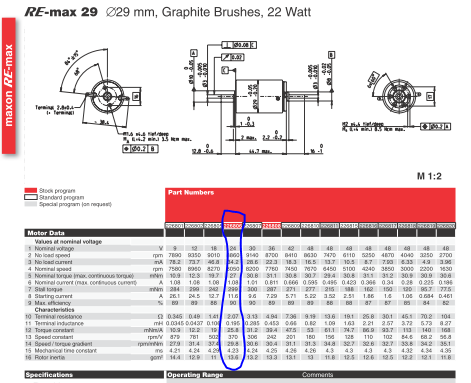
\includegraphics[scale=0.7]{Moteur.PNG}
	\caption{Moteur}
\end{figure}
\end{frame}

\begin{frame}
\frametitle{Moteur}
\begin{figure}[!ht]
	\centering
	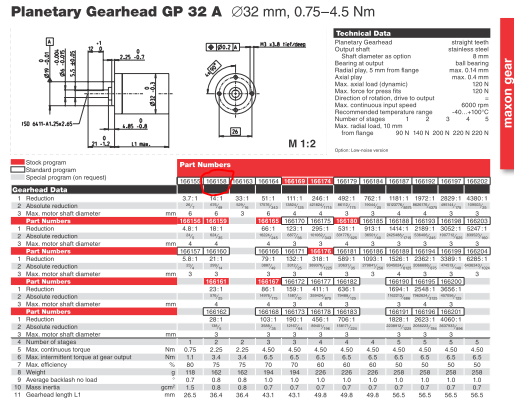
\includegraphics[scale=0.6]{Gearhead.PNG}
	\caption{Gearhead}
\end{figure}
\end{frame}

\begin{frame}
\frametitle{Moteur}
\begin{figure}[!ht]
	\centering
	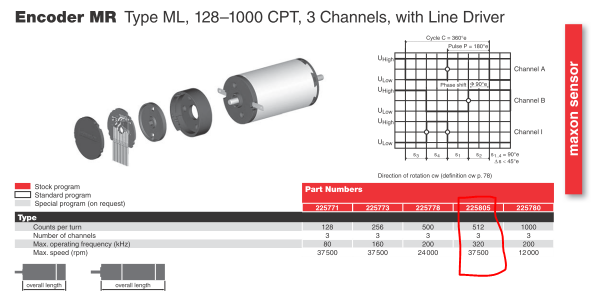
\includegraphics[scale=0.6]{Encoder.PNG}
	\caption{Encoder}
\end{figure}
\end{frame}

\begin{frame}
\frametitle{Driver}
\end{frame}
\begin{frame}
\frametitle{Perspectives}
\begin{description}
\item[OpenCV] Traitement d'image;
\item[Line Tracking] Suiveur d'une ligne;
\item[Pince] Prendre/Bouger/Monter des objets;
\item[Position] Système de position sur la table.
\end{description}
\end{frame}


\begin{frame}
\begin{center}
{\Huge Des questions ?}
\end{center}
\end{frame}

\end{document}
